\chapter{Design and Implementation}\label{ch:design}

\section{Multiplexer Policy}

We design several different multiplexers, each implementing a different policy
that only seeks to cater to specific use cases. The multiplexers are trusted components,
and thus are kept intentionally simple to leave them accessible to formal verification.
The main tasks of the multiplexers, regardless of policy implemented, are as follows:

\begin{itemize}
    \item Given a virtual address from the client/copier, translate it to a phyiscal address before
            handing it over to the driver.
    \item Given a physical address from the driver, translate it to a virtual address before
            handing it over to the client/copier.
    \item Sanitise any buffer addresses from the client before forwarding them.
    \item Sanitise any addresses from the driver. 
    \item Transmit buffers belong to the client, and therefore all free buffers on the transmit path
            must be returned to the appropriate client.
    \item Receive buffers belong to the driver, and therefore all free buffers on the receive path
            must be returned to the driver.
    \item Implement policy as detailed below.
    \item The transmit multiplexer has the ability to sanitise the ethernet header of outgoing packets
          to ensure the destination MAC address is well formed and will not cause issues
          on the network. Modern NICs are capable of sanitising headers of outgoing packets,
          but many systems may require a design whereby the NIC is not trusted to perform this check 
          and thus it should be done in software.
\end{itemize}

\subsection{Receive Policy}\label{s:rx_policy}

All incoming packets are processed in FIFO order. The multiplexer contains a 
mapping of virtualised client MAC addresses and client queues. After dequeuing an incoming packet,
the multiplexer must first invalidate the cache (to ensure subsequent reads are fetched again from memory)
and read the packet header. The packet header contains the destination MAC address and if the packet is
addressed to a client on the system, the buffer address is forwarded to the appropriate client. 
If a client's Receive Used (RxU) queue is full, the multiplexer drops the packet and the buffer address is returned to
the driver. This can be prevented for higher priority clients by appropriate choice of client's RxU queue
sizes. Appropriate sizes can be selected based on experients discussed in \autoref{ch:evaluation}.

The multiplexer must also return free buffers to the driver to be reused again. If a clients Receive Free
(RxF) queue is full, the multiplexer could stall the client while it waits to enqueue free buffers. Should this be the case,
the order in which the multiplexer processes the client RxF queue contains policy as it may
unblock clients. We propose instead to ensure the clients RxF queue is the same size as the number
of receive buffers circulating and thus prevent the client becoming blocked on waiting for this queue to be
processed. This design removes the need for policy on processing free buffers. \\ 

\subsection{Transmit Policy}

All incoming requests from clients are processed subject to a particular policy. The designs of some
example policies are outlined below.\\
The transmit multiplexer returns free buffers from the driver to the client in FIFO order.
We propose client Transmit Free (TxF) queues are at least the size of the number of buffers
belonging to that client in order to prevent the multiplexer from becoming blocked 
should a client's TxF queue become full. \\ 
Similarly, the drivers Transmit Used (TxU) queue should be at least the size of the sum of 
all client transmit buffers. This ensures the multiplexer will not become blocked on this queue
and thus disrupt the policy implemented to process client requests. \\ 

\subsubsection{Round Robin Policy}
We implement a round robin policy by processing a single client's transmit request at a time.
This is done in a loop to ensure we process any batched requests as outlined in \autoref{l:roundrobin}.

\begin{figure} [H]
    \begin{minted}[]{c}
void process_transmit_ready():
    enqueued = 0
    old_enqueued = 0

    while(!ring_full(driver.used_ring)):
        old_enqueued = enqueued
        for each client:
            /* Process a single used buffer at a time */
            if (!ring_empty(client.used_ring) &&
                !ring_full(driver.used_ring)):
                buf = dequeue(client.used_ring)
                phys = get_phys_addr(buf)

                enqueue(driver.used_ring, phys)

                enqueued += 1
            
        /* we haven't processed any packets since last loop, exit */
        if (old_enqueued == enqueued) break
\end{minted}
\caption{Transmit Round Robin Policy}
\label{l:roundrobin}
\end{figure}

\subsubsection{Priority-based Policy}

We implement a priority-based policy in \autoref{l:prioritybased}. We assume the list of
clients is ordered from highest priority to lowest. Thus it is possible to change a clients
priority at run time by manipulating this list.\\

\begin{figure} [H]
    \begin{minted}[]{c}
void process_transmit_ready():
    enqueued = 0
    old_enqueued = 0
    while(!ring_full(driver->used_ring)):
        old_enqueued = enqueued
        for client in clients:
            while(!ring_empty(client->used_ring) &&
                    !ring_full(driver->used_ring)):
                buf = dequeue(client.used_ring)
                phys = get_phys_addr(buf)
                enqueue(driver.used_ring, phys)

                enqueued += 1
                /* if a higher priority client has since 
                    made a request, go again */
                if (!ring_empty(clients[:client])): break

        if old_enqueued == new_enqueued: break
\end{minted}
\caption{Transmit Priority-based Policy}
\label{l:prioritybased}
\end{figure}

\subsubsection{Bandwidth Limited Policy}\label{s:bandwidth}

We implement a bandwidth-limited policy in \autoref{l:bandwidth}. The multiplexer will 
process client transmit requests, caluclating how much bandwidth the client has used based on
each request size in a given time window. Should a client exceed its limit within the time window,
the multiplexer will request a time out from the timer driver for the remaining time. As the multiplexer must
regularly communicate with the timer driver to get the time and set timeouts, we design a simple timer driver
API as shown in \autoref{l:timer}. 

\begin{figure} [H]
    \begin{minted}[]{c}
void process_transmit_ready():
    curr_time = get_time()
    for each client:
        if (curr_time - client.last_time >= TIME_WINDOW):
            client.last_time = curr_time
            client.bandwidth = 0
        
        while !ring_empty(client.used_ring) && 
                !ring_full(driver.used_ring) && 
                client.bandwidth < client.max:
            buf = dequeue(client.used_ring)
            phys = get_phys_addr(buf)
            enqueue(driver.used_ring, phys)
            /* recalculate the clients bandwidth used in 
                the current time period */ 
            client.bandwidth = calculate_bandwidth(buf_size)

        if !ring_empty(client.used_ring) && !client.timeout:
            set_timeout(TIME_WINDOW - curr_time - client.last_time)
            client.timeout = true
\end{minted}
\caption{Transmit Bandwidth Limited Policy}
\label{l:bandwidth}
\end{figure}

\begin{figure} [H]
    \begin{minted}[]{c}
uint64_t get_time() {
    return microkit_ppcall(TIMER, microkit_msginfo_new(GET_TIME, 0));
}
        
void set_timeout(uint64_t micros) {
    microkit_mr_set(0, micros);
    microkit_ppcall(TIMER, microkit_msginfo_new(SET_TIMEOUT, 1));
}
\end{minted}
\caption{Timer Driver API}
\label{l:timer}
\end{figure}

The timer driver is a high priority, passive server. It receives interrupts from the device,
and forwards these by notifying the appropriate client or multiplexer. The bandwidth limited
multiplexer reacts to such notifications by clearing the appropriate clients timeout and
recalling process\_transmit\_ready. Note that this implementation could be made more efficient
by mapping the timer registers read-only into the multiplexer address space. This would remove
the need for a system call that frequently gets the time. However, these implementations are 
meant only as example multiplexers rather than a prescribed implementation. \\

This bandwidth-limited policy can also be combined with the round robin or priority based policy
to order each clients requests. Such a case would be useful in reducing the 
transmit latencies of latency sensitive applications.\\ 

% does it make sense to set a total limit greater than whats actually available? 

\subsection{Enforcing Policy Through System Design}
Depending on the greater system design, we expect some transmit policies to not work.
For example, given a single-core configuration, the higher priority multiplexer will
always be invoked as soon as a client has made a request to transmit. This means that
we can assume any other clients do not yet wish to transmit, or have not yet had the
opportunity to run to make a request. Therefore, the multiplexer does not need to 
consider all the client queues when invoked and can just service requests made
by the client that signalled. To enforce policy on multiple clients in such a scenario,
we rely on appropriate choices of client queue sizes and the scheduling parameters
of each client. For example, to enforce a round robin policy on two clients, we run both clients
at equal priorities, and limit their TxU queues to just one. This ensures
that each client will be stalled until their single request has been processed, and
another client will have the opportunity to run in the interim. The multiplexer will
then only process a single request per client at a time, though at the detriment to performance.\\
Similarly, should we require a priority based policy, we can assign appropriate priorities
to the clients and limit lower priority client's queue sizes, thus relying on the scheduling
of the system to reinforce this policy.\\
Finally, we can limit the client's queue sizes on both the transmit and/or receive paths
to limit the amount of either transmit and/or receive throughput available to each client.
Appropriate sizes can be selected based on experients discussed in \autoref{ch:evaluation}.\\ 

\section{Broadcast Protocols}
Some protocols broadcast traffic to all systems by addressing the
ethernet packet with a specific MAC address of ff:ff:ff:ff. However,
as the receive multiplexer is based on MAC addresses, it will not
know how to handle such packets. In particular, we need to support 
the Address Resolution Protocol (ARP), as it maps an
IPv4 address to a MAC address and thus 
is required for any network communication via ethernet.\\
One possible solution is to copy these packets to all client applications.
This would require additional policy in the receive multiplxer that ensures
all client side RxF queues have enough free buffers available
for the multiplexer to dequeue and then copy broadcast packets into.
However, there are many different broadcast protocols, for example the Dynamic
Host Configuration Protocol (DHCP), and the arrival of such packets
can be nondeterministic. This makes it difficult to determine how many might arrive
simultaneously and thus how many buffers should be available in all client side
RxF queues at all times. If there are no any free buffers available for ARP, then
a client will not be able to receive any IPv4 traffic.\\
Instead, we implement a separate component to handle broadcast traffic. It interfaces
with the multiplexers the same as any other client, as shown in \autoref{f:mux}. 

\begin{figure}[h]
    \centering
    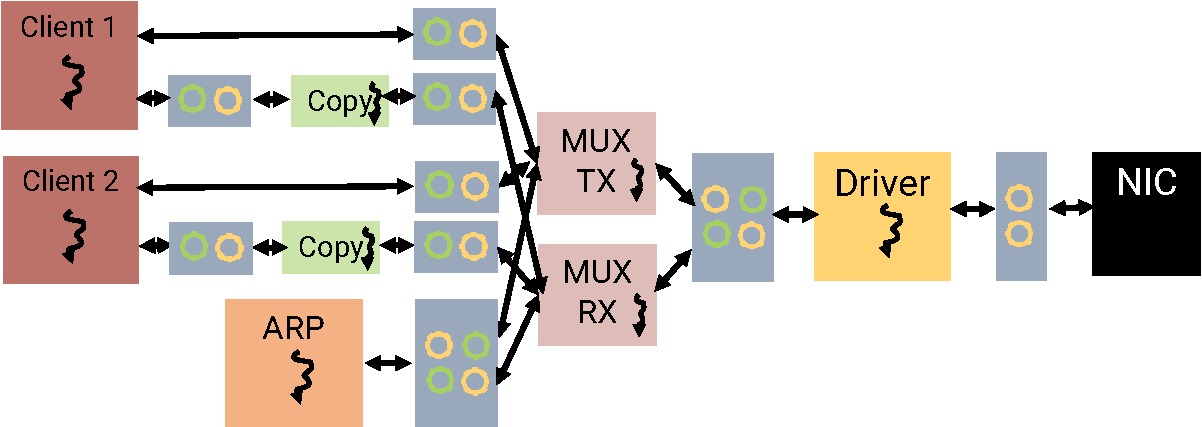
\includegraphics[width=\textwidth]{arp.pdf}
    \caption{Multiple client applications with an ARP component on the sDDF}
    \label{f:arp}
\end{figure}

\subsection{Separate ARP Component}
A separate ARP component only requries the minimal functionality to respond to 
the address resolution protocol on behalf of any client applications running on
the system. In keeping with the design goals, this component will be kept 
very simple in the aims of enabling formal verification. Therefore we consider
this component to be trusted to maintain the integrity of its shared queues with
the multiplexer components as well as interfacing with clients and responding
correctly to ARP on behalf of the clients. \\
While supporting other broadcast protocols, such as DHCP, is out of scope of this thesis, 
the simplicity of the ARP component design enables its functionality to be extended easily
to support other broadcast protocols in the future.

\subsection{Client Interface}
As ARP is based on both MAC addresses and IPv4 addresses, the new component
requires an interface with client applications. This interface will allow clients
to register a new IPv4 address, change an IPv4 address, or remove one. As adding,
changing and removing an IPv4 address is typically very infrequent for networking systems
and requires minimal data exchange, we define this interface using a protected procedure
call (PPC) from the client to the ARP component. 

\begin{figure} [H]
    \begin{minted}[]{c}
void register_ip4(new_ip4_addr, mac_addr[6])
{
    /* split the MAC address across two registers so it fits */
    microkit_mr_set(0, mac_addr[0:4]);
    microkit_mr_set(1, mac_addr[4:6]);
    microkit_mr_set(2, new_ip4_addr);
    microkit_ppcall(ARP, microkit_msginfo_new(REGISTER_IP, 3));
}

void change_ip4(old_ip4_addr, new_ip4_addr, mac_addr[6])
{
    microkit_mr_set(0, mac_addr[0:4]);
    microkit_mr_set(1, mac_addr[4:6]);
    microkit_mr_set(2, old_ip4_addr);
    microkit_mr_set(3, new_ip4_addr);
    microkit_ppcall(ARP, microkit_msginfo_new(CHANGE_IP, 4));
}

void remove_ip4(old_ip4_addr, mac_addr[6])
{
    microkit_mr_set(0, mac_addr[0:4]);
    microkit_mr_set(1, mac_addr[4:6]);
    microkit_mr_set(2, old_ip4_addr);
    microkit_ppcall(ARP, microkit_msginfo_new(REMOVE_IP, 3));
}
\end{minted}
\caption{Client Interface to ARP Component}
\label{l:arpintf}
\end{figure}

Currently, the ARP component can only store a single IPv4 address per client, which
is enough for our testing purposes, however this limit can be extended easily in the code
base should the need arise.\\

\section{Client Applications}\label{s:client_apps}

The client application consists of a simple echo server and uses lwIP \cite{Dunkels_01} as an IP
stack library to process the network packet headers. The lwIP API stores packet data, including pointers
to the payload, in a pbuf struct. The pbufs are allocated from static sized memory pools and can be chained
together. On the receive path, pbufs aren't chained together as the incoming payload already contains
all the required packet headers. However, when transmitting a packet via the UDP or TCP API, the pbuf will
only wrap around the actual payload, and in order to add the required headers, lwIP allocates additional pbufs
containing these headers that are added to the head of a pbuf chain. Once a packet is ready to be transmitted,
a chain of pbufs must then all be copied into a single sDDF buffer before being enqueued to the multiplexer.
The result of this design means that if there isn't a transmit buffer available for this chain of pbufs, the
packet is dropped and the pbufs are freed. While this is an acceptable outcome, it unfortunately means that a significant
amount of packet processing is then wasted. In order to combat this on the simple echo server and reduce
wasted cycles, packets are only
processed on the receive path depending on the availability of transmit buffers. This stalls the client application
until it receives a notification that more transmit buffers are available. \\
However, this solution is very limiting
as most networking applications do not have symmetric traffic. For example, a client application could receive a
higher number of packets than it transmits, and thus the design stalls the receive processing without reason. 
On the other hand, a client application with higher transmit demands would bypass the check for transmit buffers and result in
packets being dropped after packet processing. \\
To remove the premature check for transmit buffers on the receive path, we need to 
temporarily store the transmit context by storing the pbuf chains when there are not enough transmit buffers
available to the client. Once more transmit free buffers are available (by which the client will be notified),
the client can resume the transmit context. 

\begin{figure}[h]
    \centering
    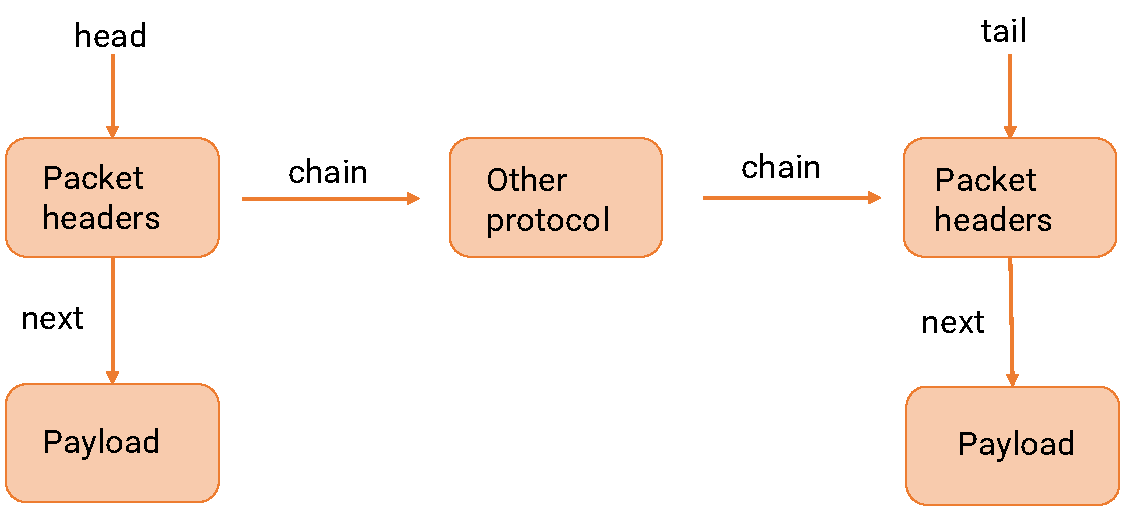
\includegraphics[width=0.8\textwidth]{pbufs.pdf}
    \caption{Example lwIP pbuf chain}
    \label{f:pbufs}
\end{figure}

We store the transmit context by simply linking pbuf chains together and storing the head and tail of the list. 
\autoref{f:pbufs} shows how multiple chains of pbufs can be linked together. When a chain of pbufs is ready to
be transmitted, but there are not any free transmit buffers, we append the chain to the tail of the list and 
increment the reference count of the chain. This ensures the pbufs won't be freed until they have actually been sent.
When a client is notified of the availability of more free transmit buffers, we dequeue pbuf chains from the head of
this list. This only requires adding a single extra field to lwIP pbuf structs. This simple change removes any
restriction on the receive path, sets up the client application to no longer expect symmetric traffic.\\

\subsection{Asymmetric Traffic}
Now that we can support assymmetric traffic in the client application, we require simple test cases that emulate different
applications that could be deployed on a real system. We wish to test
applications with different requirements: an application with higher transmit demands and minimal incoming traffic,
and an application with higher receive demands and minimal outgoing traffic. 

\subsubsection{Transmit dominant application}\label{s:transmit_dom}
We implement a simple client application that transmits 10,000 UDP packets, of 1472 bytes each, for every UDP packet received.
Ethernet maximum transmission unit is 1518 bytes, which leaves a maximum of 1472 bytes in payload once you account for 14 bytes
in ethernet headers and 32 bytes for UDP/IP headers. 
In order to interface with lwIP to initiate additional transmits, we first allocate a pbuf, and write 1472 bytes of data
to the pbuf's payload. As pbufs are allocated from a memory pool, they can also run out. Should this occur, we temporarily
pause the transmit context by storing the number of packets we have already sent so we can transmit the rest once more 
memory has freed up. The bottleneck on memory availability for lwIP pbufs occurs because pbufs are queued while the application
waits for more transmit buffers as outlined above. Thus, when transmit buffers become available, so to does more memory for
pbufs. We can thus resume the transmit context once the transmit multiplexer has notified the application that more
transmit buffers are available. The benefit of temporarily pausing the transmit context is that it also ensures the application
is available to process any incoming traffic in the interim. 

\subsubsection{Receive dominant application}
We also implement a simple receive dominant client application that for every 10,000 UDP packets received, it transmits a single one.
This application is much simpler to implement as all memory management is already dealt with so we just adapt the echo server to 
only echo every 10,000th packet.\\

\subsection{Client Initiated Transmit}
Not all networking devices act as servers that only react to incoming traffic. A common use case of a non-reactive application is a 
web client which initiates network communication with another networking device. To test such a scenario, we implement another client
application which first initiates a handshake with another device, then transmits 1,000,000 packets. The initial handshake is there to 
ensure the external benchmarking application is ready to receive all incoming packets. We interface with lwIP as described
in \autoref{s:transmit_dom}.

\subsection{Computate heavy applications}\label{s:compute_heavy}
Another limitation of the test environment is that the client applications do not actually do any processing with the incoming or outgoing traffic.
A typical networking system would perform some computation on the incoming data, such as a HTTP webserver, which would need to fetch web pages from
memory to process incoming HTTP requests. Although developing such a test scenario is out of scope for this thesis, we still want to test
our framework under high loads where the CPU cannot keep up with the traffic to ascertain the abscence of a performance collapse, as well as
ensuring that the system abides by any policy implemented in a multi-client set up. We alter the echo application to perform 10 unecessary data copies
and checksum calculations.

\section{Two-threaded driver on multicore systems}
A device driver has multiple tasks: it must react to hardware events as signalled by an interrupt and it must react to software events,
such as a client request. Namely, the driver has 4 tasks:

\begin{enumerate}
    \item Dequeue incoming packets from the hardware receive ring and enqueue them to the RxU queue.
    \item Dequeue free buffers from the RxF queue and enqueue them to the hardware receive ring.
    \item Dequeue used transmit buffers from the TxU queue and enqueue them to the hardware transmit ring.
    \item Dequeue transmitted buffers from the hardware transmit ring and enqueue them to the TxF queue. 
\end{enumerate}

While these tasks involve interfacing with both hardware and software queues, each task involes
producing/consuming to different queues and reacting to different events. Task 3 occurs after a client transmit signal, 
tasks 1 and 4 occur after an interrupt, and task 2 occurs either preemptively after task 1 to ensure the hardware receive
ring is ready to be received, or after a client signal that more free buffers are available. We can split the driver up into
two separate components and simplify the workload as shown in \autoref{f:two_threaded_driver}.

\begin{figure}[h]
    \centering
    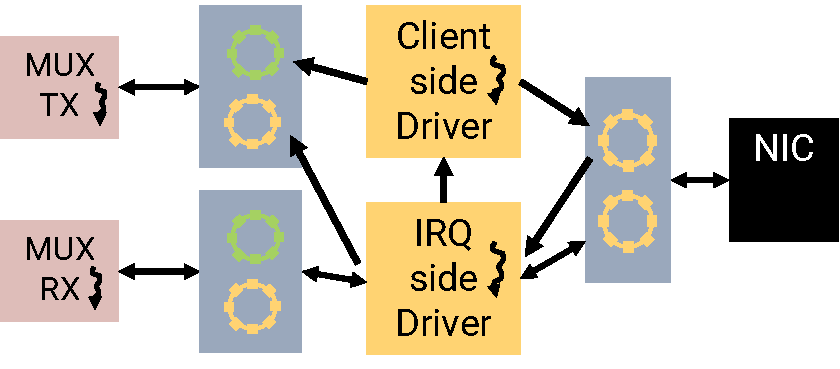
\includegraphics[width=0.6\textwidth]{two_threaded_driver.pdf}
    \caption{Driver architecture with two components}
    \label{f:two_threaded_driver}
\end{figure}

The client side driver is responsible for only task 3. It receives a signal from the transmit multiplexer when packets are ready
to be transmitted, and enqueues them to the tail of the hardware transmit ring. If the hardware transmit ring is full, it waits 
until it receives a notification from the IRQ side driver when space has freed up.\\
However, introducing an additional component to the framework will incur additional performance overheads due to extra context switches required.
We first analyse these overheads in \autoref{ch:evaluation} before concluding whether this design is appropriate on multicore systems. 

\section{Security}
One of our main design goals is to prioritise security. This means ensuring a 
misbehaving client application does not have the ability to interfere with other clients and/or the rest of the system. Clients receive
data by dequeuing metadata, including buffer addresses, from a shared ring buffer, and transmit data by enqueueing such metadata. 
However, as these shared ring buffers are used by the components on either side of the client (eg. a multiplexer), we currently 
trust the client to maintain the integrity of the queues, and not write to buffers during DMA (ie. once a packet has been enqueued
for transmit and before the buffer returns in the free queue). Specifically, we trust the client to:
\begin{enumerate}
    \item Update the tail pointer when dequeing incoming packets from its RxU queue.\\
    While the rest of this queue can be mapped in as read only to the client, if the client does not correctly increment this pointer,
    the copy component will incorrectly see this queue as full/empty and potentially could either write over client's data or stop
    enqueueing new packets. As each client application has its own copy component, this potential vulnerability is isolated only to
    the misbehaving client.
    \item Write the correct metadata to the RxF queue once buffers can be recycled.\\ 
    Should a client not do this appropriately, for example, it could give a faulty buffer address/length, the copy component will not 
    use this buffer. This vulnerability is isolated to just the client and its copy component.
    \item Update the head pointer when enqueing free buffers to its RxF queue.\\
    Like 2., this will only cause the copy component to not reuse newly enqueued buffers.
    \item Signal the copy component after enqueueing free buffers to its RxF queue.\\
    If the client does not inform the copy component of this update and the copy component is blocked on enqueueing incoming packets as there
    aren't enough free buffers to copy into, the copy component may not wake up. This could block any receive traffic to the misbehaving client
    but will not affect other components.\\
    Alternatively, if a client signals its copy component unnecessarily, this has the potential to increase networking latency. 
    As the copy component runs at higher priority than it's client, a signal from the client to its copy component will cause an immediate context
    switch. This has the potential to also affect other applications that run at equal or lower priority than the copy component on 
    the same CPU, as they may delayed to be scheduled as a result. seL4 already provides mechanisms to protect against such a scenario in 
    scheduling context objects. We can limit copy components' scheduling parameters such that they will not monopolise the CPU. Then, should 
    a client excessively signal its copier, the copy component will use up its scheduling budget and become blocked, thus reducing any Rx 
    bandwidth to that client. These limits
    will depend on greater system design, in particular, the scheduling parameters of all other applications running on the same CPU.
    \item No longer write data to buffers once enqueued to the clients RxF queue.\\
    Should the client write data to buffers already enqueued in the RxF queue, it will potentially write over incoming data. This will only
    affect the misbehaving client application, but can also be protected against by mapping Rx buffers to clients as read only.
    \item Enqueue a buffer to the RxF queue only once per use.\\
    If a client enqueues the same buffer multiple times to the RxF queue, it will potentially cause the copy component to write new incoming
    data over other used packets. This may mean the client loses Rx packets. Similarly, this will not affect any other applications.
    \item Write the correct metadata to the TxU queue.\\
    Should the client enqueue faulty metadata, such as a faulty address, the transmit multiplexer can detect this by ensuring the address lies inside
    that clients Tx DMA region, and will refuse this requeuest without impacting any other components.
    \item Update the head pointer of the TxU queue.\\
    If the client does not correctly update this pointer, the multiplexer will not see newly enqueued packets and they may never be sent.
    \item No longer write to the packet after its enqueued to the TxU queue.\\
    Should the multiplexer be responsible for ensuring the packet is well formed with appropriate ethernet headers, the client could potentially
    alter this data after sanitation and thus potentially send out corrupted packets. While modern NICs are typically equipped to prevent
    such errors, we don't want to always assume the device itself is trustworthy and corrupted packets have the potential to compromise
    other devices on the network.
    \item Signal the transmit multiplexer after enqueueing used transmit buffers.\\
    If the client does not signal the multiplexer, enqueued transmit packets may never be sent. This only affects the client itself.
    Alternatively, if the client signals the Tx multiplexer unnecessarily, it will increase latencies. Similarly to the receive path,
    a signal from client to Tx multiplexer causes an immediate context switch. Unecessarily invoking the multiplexer will delay other 
    applications running on the same core at lower priority than the multiplexer.
    \item Update the tail pointer of the TxF queue after dequeueing free transmit buffers.\\
    If this is not done and the multiplexer incorrectly sees the queue as non empty, it may write over client data and
    thus potentially overwrite and therefore lose the clients transmit requests. If
    the multiplexer incorrectly sees the queue as full, it will panic. This is because the multiplexer assumes the client's 
    TxF queues are never full (as when it dequeues a new free buffer from the driver, it cannot know in advance where 
    to return the buffer). If one client misbehaves, then it may prevent the multiplexer from dequeuing more free buffers 
    from the driver side and returning them to clients. This has the potential the corrupt the entire transmit path for all
    client applications.
    \item Enqueue a buffer to the TxU queue only once per use.\\
    If a client enqueues the same buffer multiple times to the TxU queue, it will potentially cause the device to send the
    packet multiple times. This may affect lower priority clients by monopolising the device. An appropriate choice of Tx multiplexer
    policy can protect against this consequence, and thus only affecting the misbehaving client.
    \item Keep track of all buffers.\\
    Rx and Tx buffers belong to clients and it is up to the client to not lose buffer pointers. However, should a client lose
    buffers, it could potentially limit that clients available throughput. Clients do not have access to shared buffers so this
    will not affect any other clients.
\end{enumerate}

From the above analysis, and assuming all components other than the client applications are trustworthy,
we can conclude the receive path is secure. A trusted compoent, the copier, sits between the untrusted client application
and the shared multiplexer, and in each potential vulnerability whereby the client does not abide by the protocol, the copy component
will not enqueue/dequeue more incoming packets and thus starve only the misbehaving client. This assumes the RxU queue between 
the receive multiplexer and copy component is appropriately sized. Should this queue size exceed the number of shared buffers
available for all clients, and a client misbehaves, it could potentially starve other clients. This is because the copier
of a misbehaving client will not enqueue more incoming packets to the client (either temporarily or permanently), and the RxU queue
to the copier could then fill up. If there are limited shared buffers available and a high proportion are enqueued to the copier
of a faulty client, there will be less buffers available for other clients. To prevent such a scenario, we ensure there are enough
shared buffers on the receive path for all RxU queues between the multiplexer and each copy component to be full at the same time.\\

However, the transmit path is not protected from misbehaving client applications. While scenarios 7, 8 and 13 only impact the client
itself, scenario 7 has the potential to compromise other devices on the network without a trusted device, and scenario 9 can block
all transmit traffic, including that of other clients.\\

\subsection{Transmit Copy Component}

To remove these vulnerabilities, we can mimic the receive path by injecting a small, trusted component in between each untrusted
client application and the shared multiplexer as shown in \autoref{f:tx_copy}. The component can be configured as
per the system design, or even removed all together, as required by the threat scenario.

\begin{figure}[h]
    \centering
    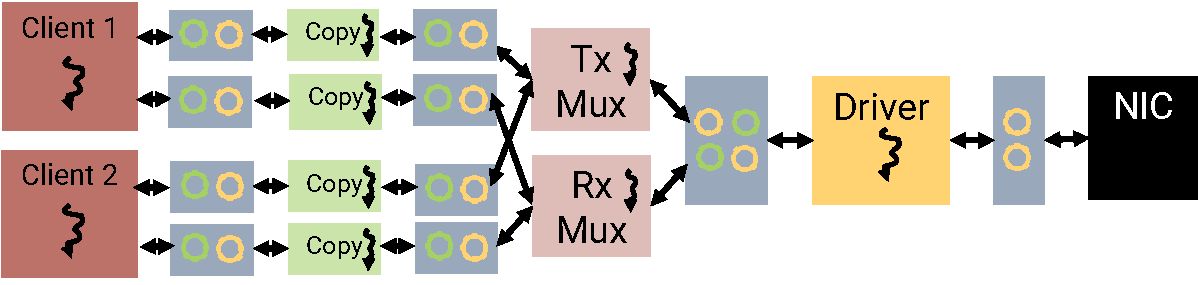
\includegraphics[width=\textwidth]{tx_copy.pdf}
    \caption{Architecture with an additional transmit copy component}
    \label{f:tx_copy}
\end{figure}

To interface with a completely untrusted client application, this new component needs to:
\begin{itemize}
    \item Ensure metadata enqueued to the multiplexer is sane.
    \item If the device is untrusted, check outgoing packets are well-formed and copy them into a separate region not mapped
          into the clients address space.
    \item Interface with the multiplexer correctly by incrementing the head/tail pointers as required.
    \item Ignore any transmit packets that do not abide by the protocols outlined above.
\end{itemize}

Like the receive path copy components, should a client misbehave when interacting with the shared queues, or fail to signal as per
the protocol, the new Tx Copy component will ignore any requests or no longer enqueue free buffers to the client, thus only disturbing
that client and not affecting any other components in the system.\\
This additional component would introduce some additional performance overheads. These include the cost of reading packet headers, 
an extra system call on the transmit path, and potentially the cost of copying the entire packet. 
We analyse these overheads in \autoref{ch:evaluation}.\\
